\section{Introduction}
\label{sec:introduction}

%{\color{blue} In this section we will contextualize video streaming technology and hierarchical caching problems, emphasizing the need of create a hierarchical topology to , and describe the content of each section of the paper.}

% Introduction of the Content and MEC service provider  
Over the years, Internet traffic has grown exponentially around the world. Mainly, due to the multimedia content streaming which, currently, represents 70\% of the whole traffic~\cite{cisco:forecast}. To deliver a video, the Video-on-Demand services generate the streaming to be distributed by the Over-The-top providers. One important point addressed by the providers is to satisfy the quality of experience~(QoE) to a wide range of users subscribers. And to provide the best user satisfaction, advantages of the high datarate and low latency in the edge network take into account nowadays~\cite{gamaUCC2019,DBLP:CoRR:2021,ye:ITC17}. This trend imposes new challenges in providing videos with the best QoE, originally designed considering the best-effort internet model for data transmission
%In this way, caching the video closer to the end-user has a positive impact on the QoE performances.

In the moment that the content provider saturates available bandwidth or a particular set of service metrics across the network, the cloud server can reroute active connections to one or more edge caches that attend to the demand required. Such model can be represented by network organized hierarchically in multi-tiers to maintain a low traffic load~\cite{rosarioSENSORS2018}.
%When the content provider saturates the available bandwidth or a certain set of service metrics, the request may be routed to one or more edge caches. This model may be organized hierarchically in multi-tiers maintains a low traffic load~\cite{rosarioSENSORS2018}.

% Challenges
As well as the advantages of using the edge of the network with cache capabilities help user satisfaction, but it could bring negative impacts as well. When many users start to request video segments at the edge nodes, these surrogated nodes consider static users and just one edge node tiers. These nodes are not ready to deal with the constant changes in the number of users and the process of switching between different Access Points~(AP) due to user mobility.
Several works in the literature highlight edge/cloud computing to deal with the new video traffic demands, but there are aspects little addressed in user dynamic solutions. Figure~\ref{fig:multi-tier-network} depicts a multi-tier network architecture, which is composed of a heterogeneous set of devices and applications using distributed computing resources through multi-access communication technology, such as 5G and WiFi.
%
%Furthermore, the number of users connected in different APs changes accordingly to the surrogated edge nodes. For instance, a core network regional edge node provides video streaming to more users than an edge gateway. As shown in Fig.~\ref{fig:multi-tier-network}.
%
%Since the triggered video segments caching (replication) in an edge node.
%However, certain precautions when choosing the nodes for caching the video need to be taken into account. 

%Which it could result some issues. 

\begin{figure}
    \centering
    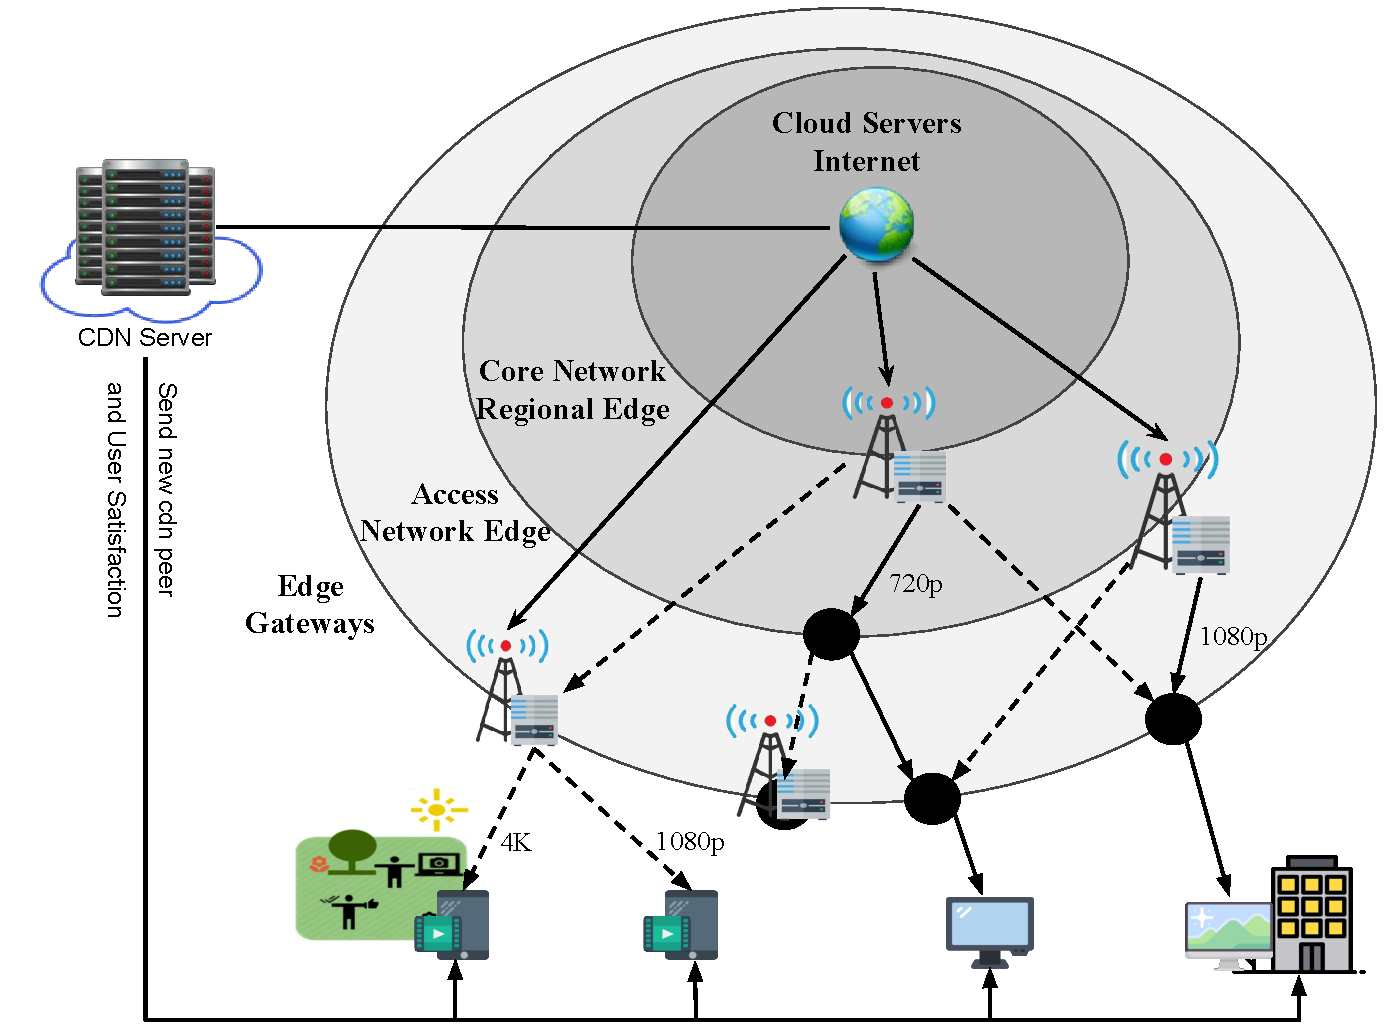
\includegraphics[width=0.9\linewidth]{images/arch-video-content.pdf}
    \caption{A General Overview of the multi-tier network environment.}
    \label{fig:multi-tier-network}
\end{figure}

% Objective
Motivated by these characteristics of multi-tier edge/cloud scenarios to improve users' satisfaction, as well as acommodate video traffic grows exponentiy. This article presents the need to have an orchestrator for the provision of video streaming content.
Our goal is to provide designers and operators a performance analysis of a hierarchical edge network and its impacts on the users' QoE. The models we present in this paper are evaluated by a series of simulations using a controlled environment.

% Organization paper
This work is organized as follows.
Section \ref{sec:related-work} presents related work on the impact of edge/cloud network on video streaming services.
Section \ref{sec:system-archi} briefly describes the proposed muti-tier edge/cloud network.
Section \ref{sec:results} shows a preliminarly results on the impact of the network performance for video streaming services.
Finally, \ref{sec:conclusion} concludes the paper.